\section{2019年国赛-线路负载及故障检测装置}
\subsection{方案总览}
总结题目要求,基本上有这几方面:

\begin{enumerate}
  \item \label{itm:l1} 负载开路、短路检测
  \item \label{itm:l2} 单元件(R、L、C)值测量
  \item \label{itm:l3} 负载网络结构检测(任意2、3个元件并联或串联)
  \item \label{itm:l4} 短路故障点距离测量
\end{enumerate}

要求\Cref{itm:l1}可通过判断ADC通道上的电压来实现,如果电压接近设计最大值,则短路,如果接近0,
则开路。

要求\Cref{itm:l2}的电阻测量,以及要求\Cref{itm:l4}中,只需看作一个电阻直接接到直流电源上,
则可通过简单的分压关系计算阻值。

要求\Cref{itm:l2}的L、C测量,可以通过信号源产生固定频率的正弦波加到负载上,
然后测量两个正交通道电压,利用相量法计算。

要求\Cref{itm:l4}的负载检测,需要具体分析各种元件串并联结构的幅频响应曲线后,
再设计相应的扫频流程,当然也可以直接按固定模式扫频获得响应曲线后再进行检测,但效率就相对较低了。

\subsection{单元件测量}
对于电阻测量,待测网络可等效为如下电路模型:

\begin{center}
\begin{circuitikz}
\draw (0,0) to[battery] (2,0) to[R, l_=$r$] (5,0) -- (5,3)
            to[R, l_=Network] (0,3) -- (0,0);
\end{circuitikz}
\captionof{figure}{直流模式下待测网络}
\end{center}

即等效为一个电阻直接接到直流电源两端,测出负载上的电压,利用串联分压计算其电阻值。

\begin{equation}
  R = \frac{V_x}{U-V_x}\cdot r
\end{equation}

以上模型也能直接用于短路故障点距离检测。

测量交流元件时,我们需要分别测量被测阻抗两端电压$V$的同相分量$V_x$和正交分量$V_y$,
计算出电压的幅度$|V|$与幅角$\theta_V$:

\begin{equation}
\begin{aligned}
  |V| &= \sqrt{V_x^2+V_y^2}\\
  \theta_V &= \arctan\frac{V_y}{V_x}
\end{aligned}
\end{equation}

由此计算出被测阻抗的幅值$|Z|$和阻抗角$\theta_Z$:

\begin{equation}
\begin{aligned}
  |Z| &= \frac{|V|}{|I|}\\
  \theta_Z &= \theta_V-\theta_I
\end{aligned}
\end{equation}

\subsection{负载网络幅频响应分析}
两个、三个元件串并联的情况列举如下(3个元件的情况下,题目只要求全部并联或全部串联)。
为了便于检测,按直流电阻值DCR的大小来划分这几种情况:

\begin{table}[H]
\center
\begin{tabular}{c|cccc}
    \hline
    DCR值 & 名称 & 图中编号 & 描述 & 幅频单调性\\
    \hline
    \multirow{3}{*}{0} & R-L par & 2 & RL并联 & 单增\\
                       & L-C par & 6 & LC并联,含ESR & 谐振峰\\
                       & RLC par & 8 & RLC并联 & 谐振峰\\
    \hline
    \multirow{2}{*}{有限非零值} & R-L ser & 1 & RL串联 & 单增\\
                              & R-C par & 4 & RC并联 & 单减\\
    \hline
    \multirow{3}{*}{$\infty$} & R-C ser & 3 & RC串联 & 单减\\
                              & L-C ser & 5 & LC串联,含ESR & 反谐振峰\\
                              & RLC ser & 7 & RLC串联 & 反谐振峰\\
    \hline
\end{tabular}
\captionof{table}{RLC网络组合情况}
\end{table}

如下是使用MATLAB画出的各种情况下的频率响应图(矢量图可放大):

\begin{figure}[H]
\center
    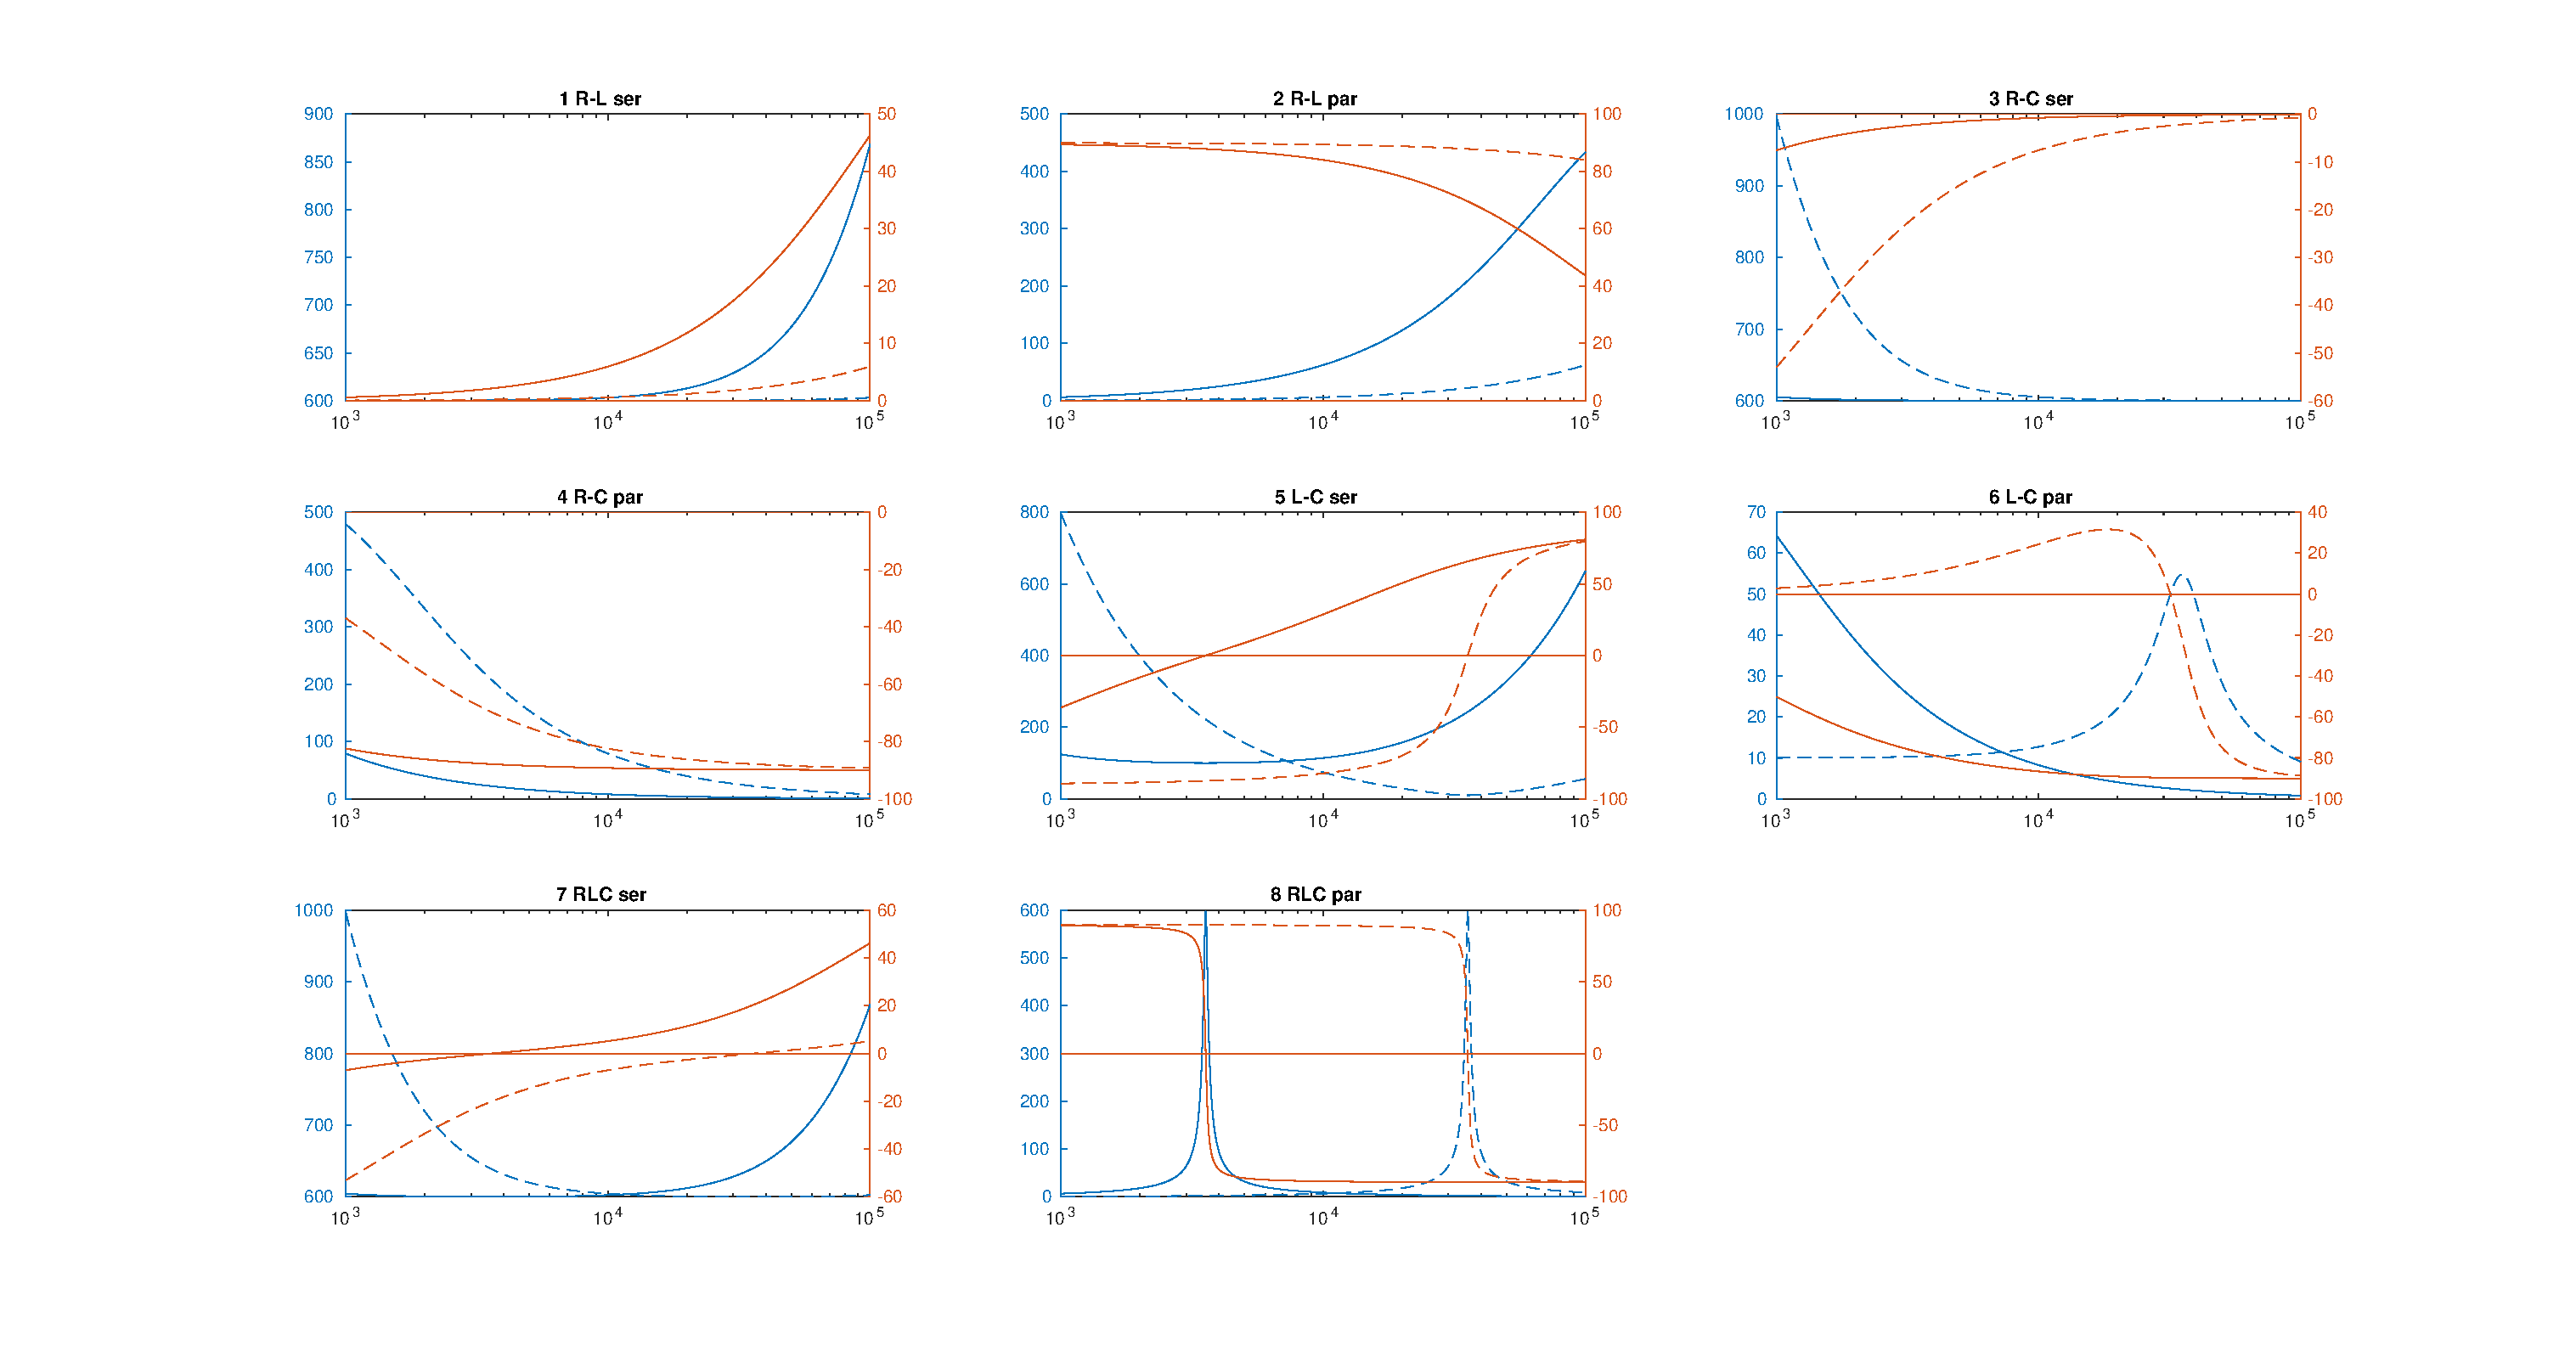
\includegraphics[width=\textwidth]{img/transfer.eps}
    \captionof{figure}{各种情况的频响曲线}
\end{figure}

图中实线、虚线分别为L,C各自取最大、最小值时的情况,方便我们分析曲线特点以及边界情况。
实际测量中,曲线不会这么极端。

因为在扫频开始前我们便能确定网络的DCR,因此针对这3种网络,分别制定相应的扫频策略:

\begin{center}
\begin{tikzpicture}[node distance=2.5cm]
\node (start)    [startstop] {DCR=0,开始};
\node (highfreq) [process, below of=start] {检查最高频率};
\node (ispos)    [decision, below of=highfreq, yshift=-0.5cm] {相位大于0?};
\node (ans2)     [io, right of=ispos, xshift=2cm] {输出结果``2''};
\node (lowfreq)  [process, below of=ispos, yshift=-0.5cm] {低频向上扫};
\node (isinc)    [decision, below of=lowfreq, yshift=-0.5cm] {相位单增?};
\node (ans6)     [io, right of=isinc, xshift=2cm] {输出结果``6''};
\node (ans8)     [io, below of=isinc, yshift=-1cm] {输出结果``8''};
\node (end)      [startstop, below of=ans8] {结束};
\draw [flarrow] (start)    -- (highfreq);
\draw [flarrow] (highfreq) -- (ispos);
\draw [flarrow] (ispos)    -- node[anchor=south] {yes} (ans2);
\draw [flarrow] (ispos)    -- node[anchor=east]  {no}  (lowfreq);
\draw [flarrow] (lowfreq)  -- (isinc);
\draw [flarrow] (isinc)    -- node[anchor=south] {yes} (ans6);
\draw [flarrow] (isinc)    -- node[anchor=east]  {no}  (ans8);
\draw [flarrow] (ans2)     |- ([xshift=2.5cm,yshift=-1cm]ans2.south east) |- (end);
\draw [flarrow] (ans6)     |- (end);
\draw [flarrow] (ans8)     -- (end);
\end{tikzpicture}
\captionof{figure}{DCR为0时扫频策略}
\end{center}

\begin{center}
\begin{tikzpicture}[node distance=2.5cm]
\node (start)    [startstop] {DCR=x,开始};
\node (highfreq) [process, below of=start] {检查最高频率};
\node (ispos)    [decision, below of=highfreq, yshift=-0.5cm] {相位大于0?};
\node (ans1)     [io, right of=ispos, xshift=2cm] {输出结果``1''};
\node (ans4)     [io, below of=ispos, yshift=-1cm] {输出结果``4''};
\node (end)      [startstop, below of=ans4] {结束};
\draw [flarrow] (start)    -- (highfreq);
\draw [flarrow] (highfreq) -- (ispos);
\draw [flarrow] (ispos)    -- node[anchor=south] {yes} (ans1);
\draw [flarrow] (ispos)    -- node[anchor=east]  {no}  (ans4);
\draw [flarrow] (ans1)     |- (end);
\draw [flarrow] (ans4)     -- (end);
\end{tikzpicture}
\captionof{figure}{DCR为非零有限值时扫频策略}
\end{center}

\begin{center}
\begin{tikzpicture}[node distance=2.5cm]
\node (start)    [startstop] {DCR=$\infty$,开始};
\node (highfreq) [process, below of=start] {检查最高频率};
\node (ispos)    [decision, below of=highfreq, yshift=-0.5cm] {相位大于0?};
\node (ans3)     [io, right of=ispos, xshift=2cm] {输出结果``3''};
\node (chkthrs)  [decision, below of=ispos, yshift=-2cm] {相位大于阈值?};
\node (ans7)     [io, right of=chkthrs, xshift=2cm] {输出结果``7''};
\node (ans5)     [io, below of=chkthrs, yshift=-1.5cm] {输出结果``5''};
\node (end)      [startstop, below of=ans5] {结束};
\draw [flarrow] (start)    -- (highfreq);
\draw [flarrow] (highfreq) -- (ispos);
\draw [flarrow] (ispos)    -- node[anchor=east]  {yes} (chkthrs);
\draw [flarrow] (ispos)    -- node[anchor=south] {no}  (ans3);
\draw [flarrow] (chkthrs)  -- node[anchor=east]  {yes} (ans5);
\draw [flarrow] (chkthrs)  -- node[anchor=south] {no}  (ans7);
\draw [flarrow] (ans3)     |- ([xshift=2.5cm,yshift=-1cm]ans3.south east) |- (end);
\draw [flarrow] (ans7)     |- (end);
\draw [flarrow] (ans5)     -- (end);
\end{tikzpicture}
\captionof{figure}{DCR无穷大时扫频策略}
\end{center}

需要注意的是,DCR无穷大情况下5(LC串联)和7(RLC串联)的区分。两者不同之处仅在于电路Q值,
因此理论上可以通过看相频在零点附近的导数大小来区分。更简单地,可以看最高频率处的相位大小来区分。
上面频响曲线的计算过程考虑了电感的ESR,是根据实测值拟合的,应该比较可靠。

\subsection{器件配置}
\subsubsection{AD9854}
在本题中我们需要使用信号源对待测网络进行扫频,根据频率和相应采集到的电压进行计算,
因此将AD9854配置为单频模式,方便灵活控制频率;由于输出接到后级运放,因此不需要OSK功能。
同时为避免高频时出现欠采样,启用PLL并设置到4倍频
(板上晶振$\SI{30}{MHz}\times 4 = \SI{120}{MHz}$)

在程序里如下配置:

\begin{cbox}{ad9854.c}
  /* 外部更新 */
  ad9854_set_bits(ad9854_updclk, ad9854_updclk_external);
  /* 单频模式 */
  ad9854_set_bits(ad9854_mode, ad9854_mode_single);
  /* 旁路反Sinc滤波器 */
  ad9854_set_bits(ad9854_invsinc_byp, 1);
  /* 关闭输出键控 */
  ad9854_set_bits(ad9854_osk_en, 0);
  /* 启用PLL */
  ad9854_set_bits(ad9854_pll_bypass, 0);
  /* 200MHz以上需设为1 */
  ad9854_set_bits(ad9854_pll_range, 1);
  /* 4倍频,经测试至少能稳定输出至50MHz而不出现欠采样 */
  ad9854_set_bits(ad9854_pll_mult, 4);
\end{cbox}

在测试阶段尝试过10倍频($\SI{30}{MHz}\times 10 = \SI{300}{MHz}$,
即AD9854最大可设置的SYSCLK频率),但会出现功耗过大的问题,
甚至偶尔会出现复位失败无输出的现象,因此综合起见,倍频在6以内比较合适。

\subsubsection{ADS124S08}
由于我们的扫频策略相对灵活,因此选择了数据驱动型的程序架构,每取得一个ADC采样数据,
就运行一次相应的事务函数,并由该函数决定是否继续采样。因此,配置ADC如下:

\begin{cbox}{measure.c}
  /* 单次转换模式 */
  ads124s_update_value(ads124s_conv_mode, ads124s_mode_single);
  /* 关闭PGA */
  ads124s_update_value(ads124s_pga_en, 0);
  /* 启用状态字节 */
  ads124s_update_value(ads124s_status_byte_en, 1);
\end{cbox}

ADC的转换开始信号START/SYNC由函数\cinl{measure_task_poll}负责拉低/置高,
保证了程序流程的同步性。
